% !TEX root = ../../thesis.tex
\tikz[remember picture,overlay] \node[inner sep=0pt] at (current page.center){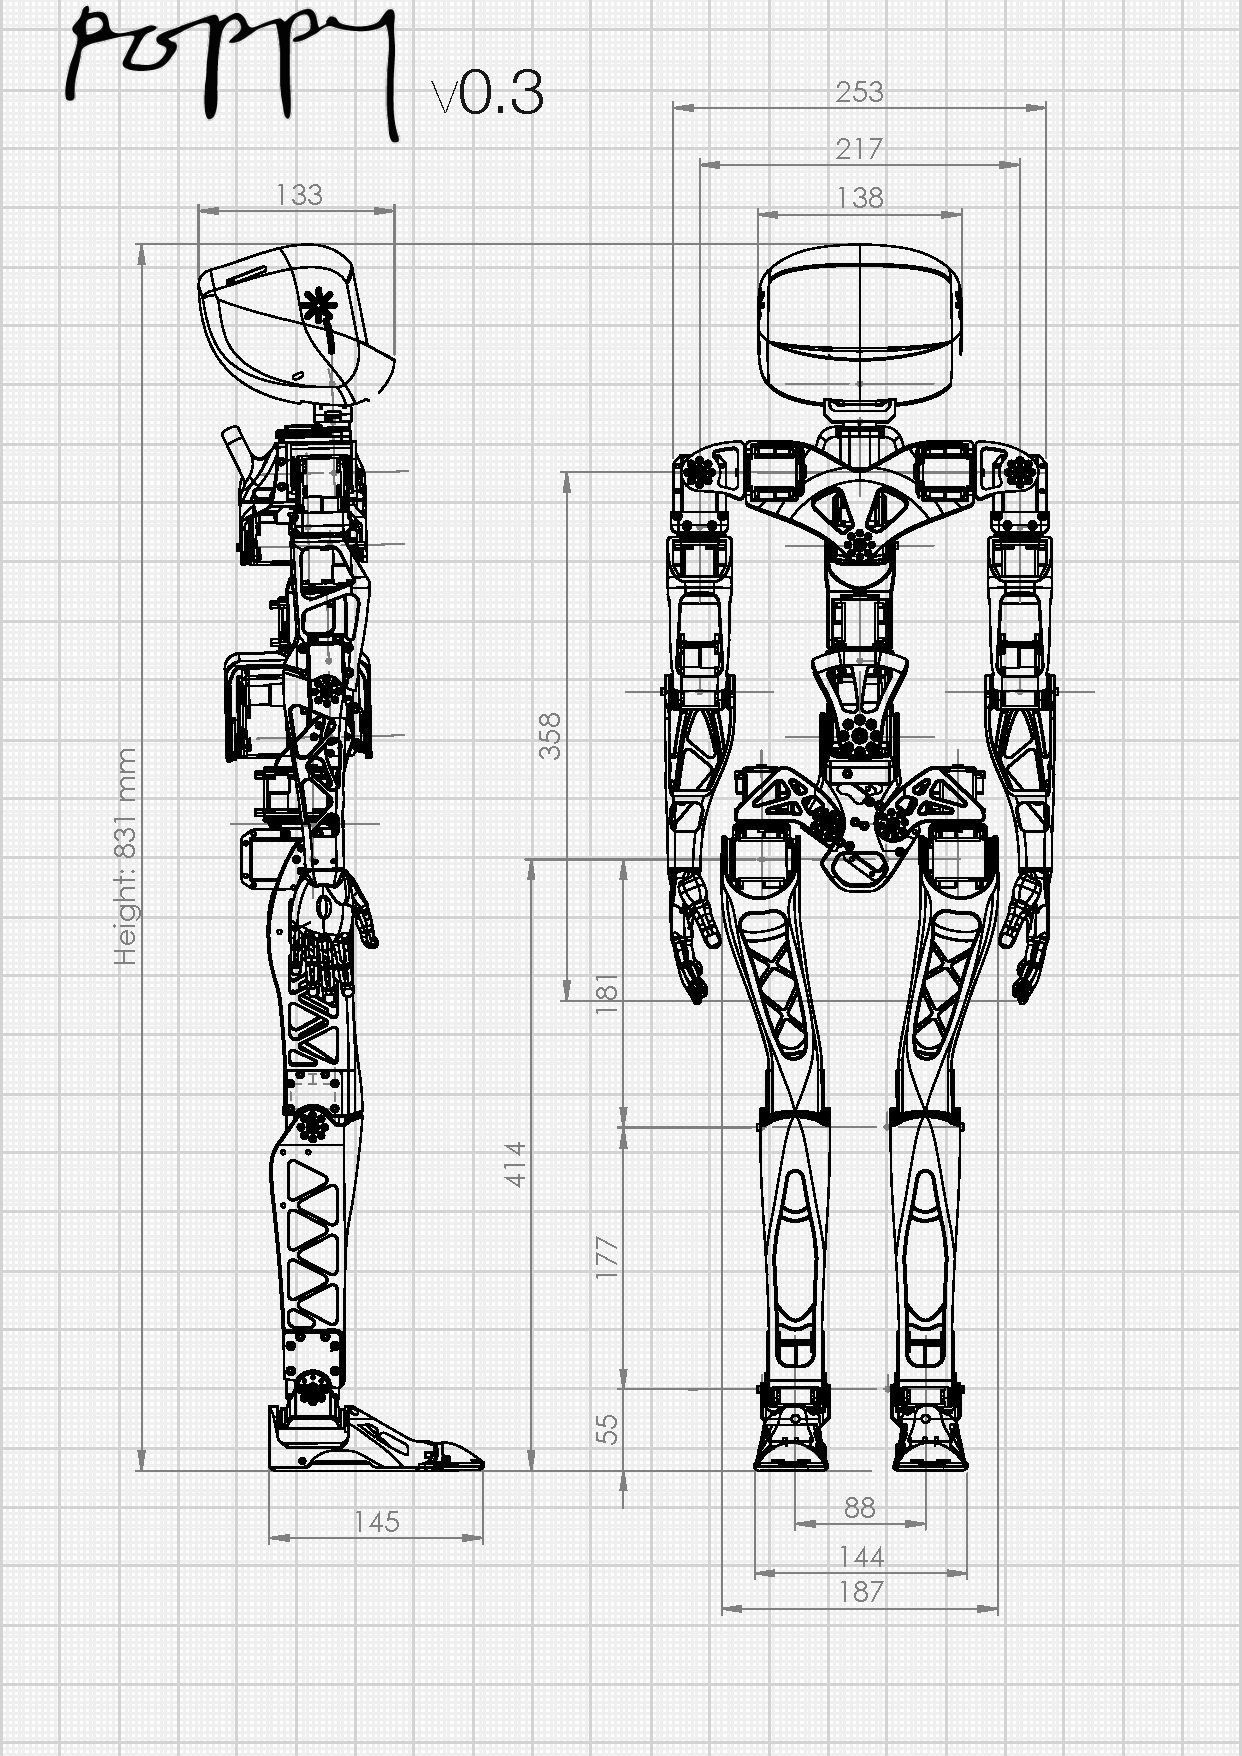
\includegraphics[width=\paperwidth,height=\paperheight]{Poppy_dimensions}};
\clearpage

\section{A little robot} % (fold)

To reach the goals presented in the introduction, the size of the robot is a really important aspect.

On one hand, small size makes the integration of complex, powerful and accurate mechatronics very difficult. Therefore it reduces the scope of technology we could use for the robot. In particular, the integration of hydraulic and pneumatic actuators, as well as advanced mechanisms involving several moving parts is really challenging.

On the other hand, having a small robot is indeed really convenient for exploring morphological properties in the real world.

Firstly, it changes significantly the experimental process: the ratio between weight, and thus energy and torques enforced by movements, and the mechanical robustness of the structure and of the actuators, is such that the robot can fall without breaking itself. Moreover, it is lightweight, which allows people to handle it directly without additional infrastructure and in a safe way. On the one hand, all of this speeds up the experimental process. On the other hand, it deeply changes the methodology of movement and motor skill design by allowing the creation of movements directly on the robot by real-world experiments without a simulation process. This includes for instance adjusting motor primitives in real time, even extreme ones

Secondly, this brings advantages regarding human interaction, which is an important focus in this work: on one hand, from the above reasons, this rules out the problem of physical security in Human/Robot interaction. On the other hand, the size of the robot plays an important role in the psychological representation that people have of it.

However exploring morphological properties requires having a robot whose morphology has an actual impact on its dynamic. Being too small reduces this impact because it reduces the inertia and the role of intrinsic structural frequency.

Thus Poppy's size is a compromise to facilitate at the same time easy testing in the real world, the integration of a large number of degrees of freedom (25 DoFs) and a structure whose dynamic properties cannot be neglected.


\section{Bio-inspired morphology} % (fold)

In the previous sections we described the global techniques and guidelines we used for building a novel humanoid robot, especially its lightness and modular morphology. In this section we will describe how we actually designed Poppy's body.

As we are especially interested by exploring and understanding the role of morphology for cognition and complex tasks achievement, among the open ended possibilities to actually create a humanoid robot, we decided to explore bio-inspired morphology. Indeed, it appears the Evolution have found several tricks permitting animals to act robustly and efficiently in the real world without requiring complex explicit computation.

We therefore decided to design the initial Poppy's body following bio-inspiration principles. In this direction, the human body appears as a good and relevant starting point. Yet a direct transposition from human body to robot morphology does not seem an effective way as the mechanical properties of biological material such as bones and muscles are very different from the technology we have in robotics. Thus we preferred take only the functional inspiration i.e. mimicking the mechanism/system properties rather than the actual morphology.

This bio-inspiration is expressed on the whole structure of Poppy and as a central challenge for humanoid robot is the biped walking, this functional bio-inspiration is mainly expressed on the locomotive system (legs and trunks) in order to increase the robot robustness, agility and stability during the walking.


\subsection{Morphological proportions} % (fold)

On the anatomical point of view, Poppy reproduces the human proportions as described in the literature~\parencite{dufour2005biomecanique} (see Fig. 3) and the sensorimotor space organization: i.e. the main degrees of freedom (actuated and passive).

While the human grows from child to adult, his body proportions change~\parencite{REF}. An hypothesis we made is that the human proportions converge toward an optimal link ratio. Based on this hypothesis we decided to respect the human body proportion of an adult thus the size of the robot describes previously (see section REF) has defined all\footnote{An exception was made for the head, which is bigger to make it more cute and will be discussed in the section REF.} Poppy's links dimensions following the proportions presented on \figurename~\ref{fig:poppy-human-proportion}.

\begin{figure}[tb]
    \begin{center}
        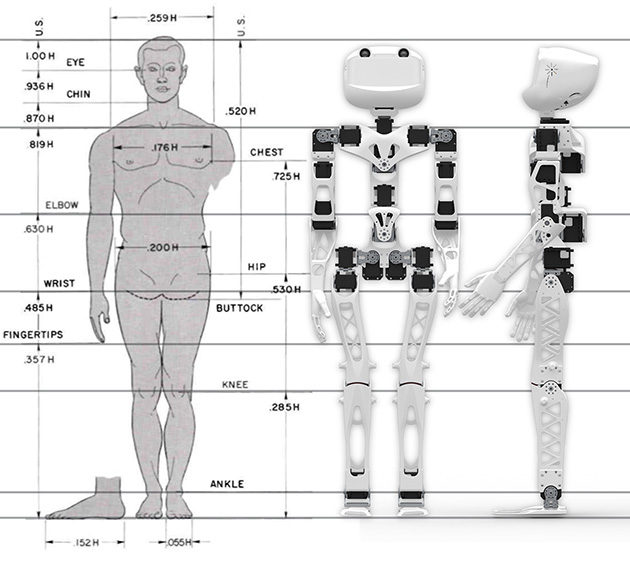
\includegraphics[width=0.8\linewidth]{proportion_poppy.jpg}
    \end{center}
    \caption{Caption here}
    \label{fig:poppy-human-proportion}
\end{figure}

Of course, this hypothesis is contestable, and as example, mimicking the proportions of a child having the same size of Poppy could be as relevant. Yet this choice has been done as a starting point, thanks to design methodology we have and the open source diffusion, anyone can easily explore other choices and compare them.

\subsection{Small and lightweight feet} % (fold)

Toward the achievement of biped locomotion, most humanoid robots have big, flat and rectangular feet. This design is indeed really convenient to simplify balance problem while it permits to increase easily the sustentation polygon, but this design choice implies some constraints:

First, increasing the foot size increases the lever arm applied to the ankle. It can be useful as it extends the impact of the ankle control over the whole body. Yet given the potential high-torque applied to the ankle, achieving such control requires very powerful actuator.
Powerful actuators are heavier and therefore the whole actuation design of the robot needs to be powerful in order to be able to lift and move the feet.

Secondly, some interesting dynamic controllers for biped locomotion seems require mass-less legs~\parencite{REF}. Indeed, in this case there is no inertia moment due to the legs motions, therefore controlling the whole body is simplified. While this case is a theoretical trick, it can still be transfered in the real world by having a strong trunk/legs mass ratio. Therefore, either the global mass of the robot should increases in order to make the mass of leg negligible or we should design more lightweight legs.
Because they are the most éloigné element from the trunk, the mass of the feet has a strong impact on the leg inertia.

Finally, while current state of the art, shows that it stills more simple to have big and heavy foot\parencite{REF} to achieve biped locomotion, some works show impressive results thanks to the use of small feet or flexible feet~\parencite{bruneau2001dynamic}. We can cite in particular Petman (see figure REF) those demonstrates breaking-edge skills for biped locomotion over very complex terrain\footnote{Link youtube}.
Moreover this aspect seems to be coherent with the multi-legged animals kingdom, indeed most of animals have really thin legs and very small feet (see fig REF).

So even if common humanoid robots still use big and powerful feet, for the above mentioned reasons, we decided to explore bio-inspired, small, and lightweight feet.

While the human foot is very complex system involving dozens of bones, muscles and tendons, we simplified the design by extracting few relevant functional human foot properties such as toes, which are key features concerning both the human walking~\cite{Hughes1990} and biped robots with a human-like gait~\cite{Sellaouti2006}. On the Poppy's feet, to reduce the weight and complexity, we designed a passive articulation with torsion spring (see figure REF).
Also Poppy has very small foot compare to common humanoids, the height/foot's length ratio is close to the human one with about 17\% while robot such as Nao have feet represents 27\% of its height (see table REF).

\begin{table}[h]
\centering
\begin{tabular}{l| c c c c c}
    & Human & Nao & Darwin Op & Nimbro-OP & Poppy \\
    \hline
    height (cm) & NA & 58 & 45 & 20 & 83\\
    Foot length (cm) & NA & 16 & 23 & 20 & 14.5\\
    ratio (\%) & 16 & 27 & 23 & 20 & 17\\
\end{tabular}
\caption{}
\label{tab:poppy_feet_compare}
\end{table}

Finally, unlike most humanoids, Poppy has only one active DoF. Indeed, while Poppy has small feet, it appears the actual moment it can transmit to the ground is really little for the lateral motion. Also creating an active articulation would add a lot of mass (72 gr) for little actual effect. Yet this DoF is still useful for ground adaptation. We therefore prefered to design an articulation based on a passive joint with torsion springs (see fig REF).


% \begin{figure}[tb]
% \centering
%     \subfloat[][]{\label{fig:frontal_trunk}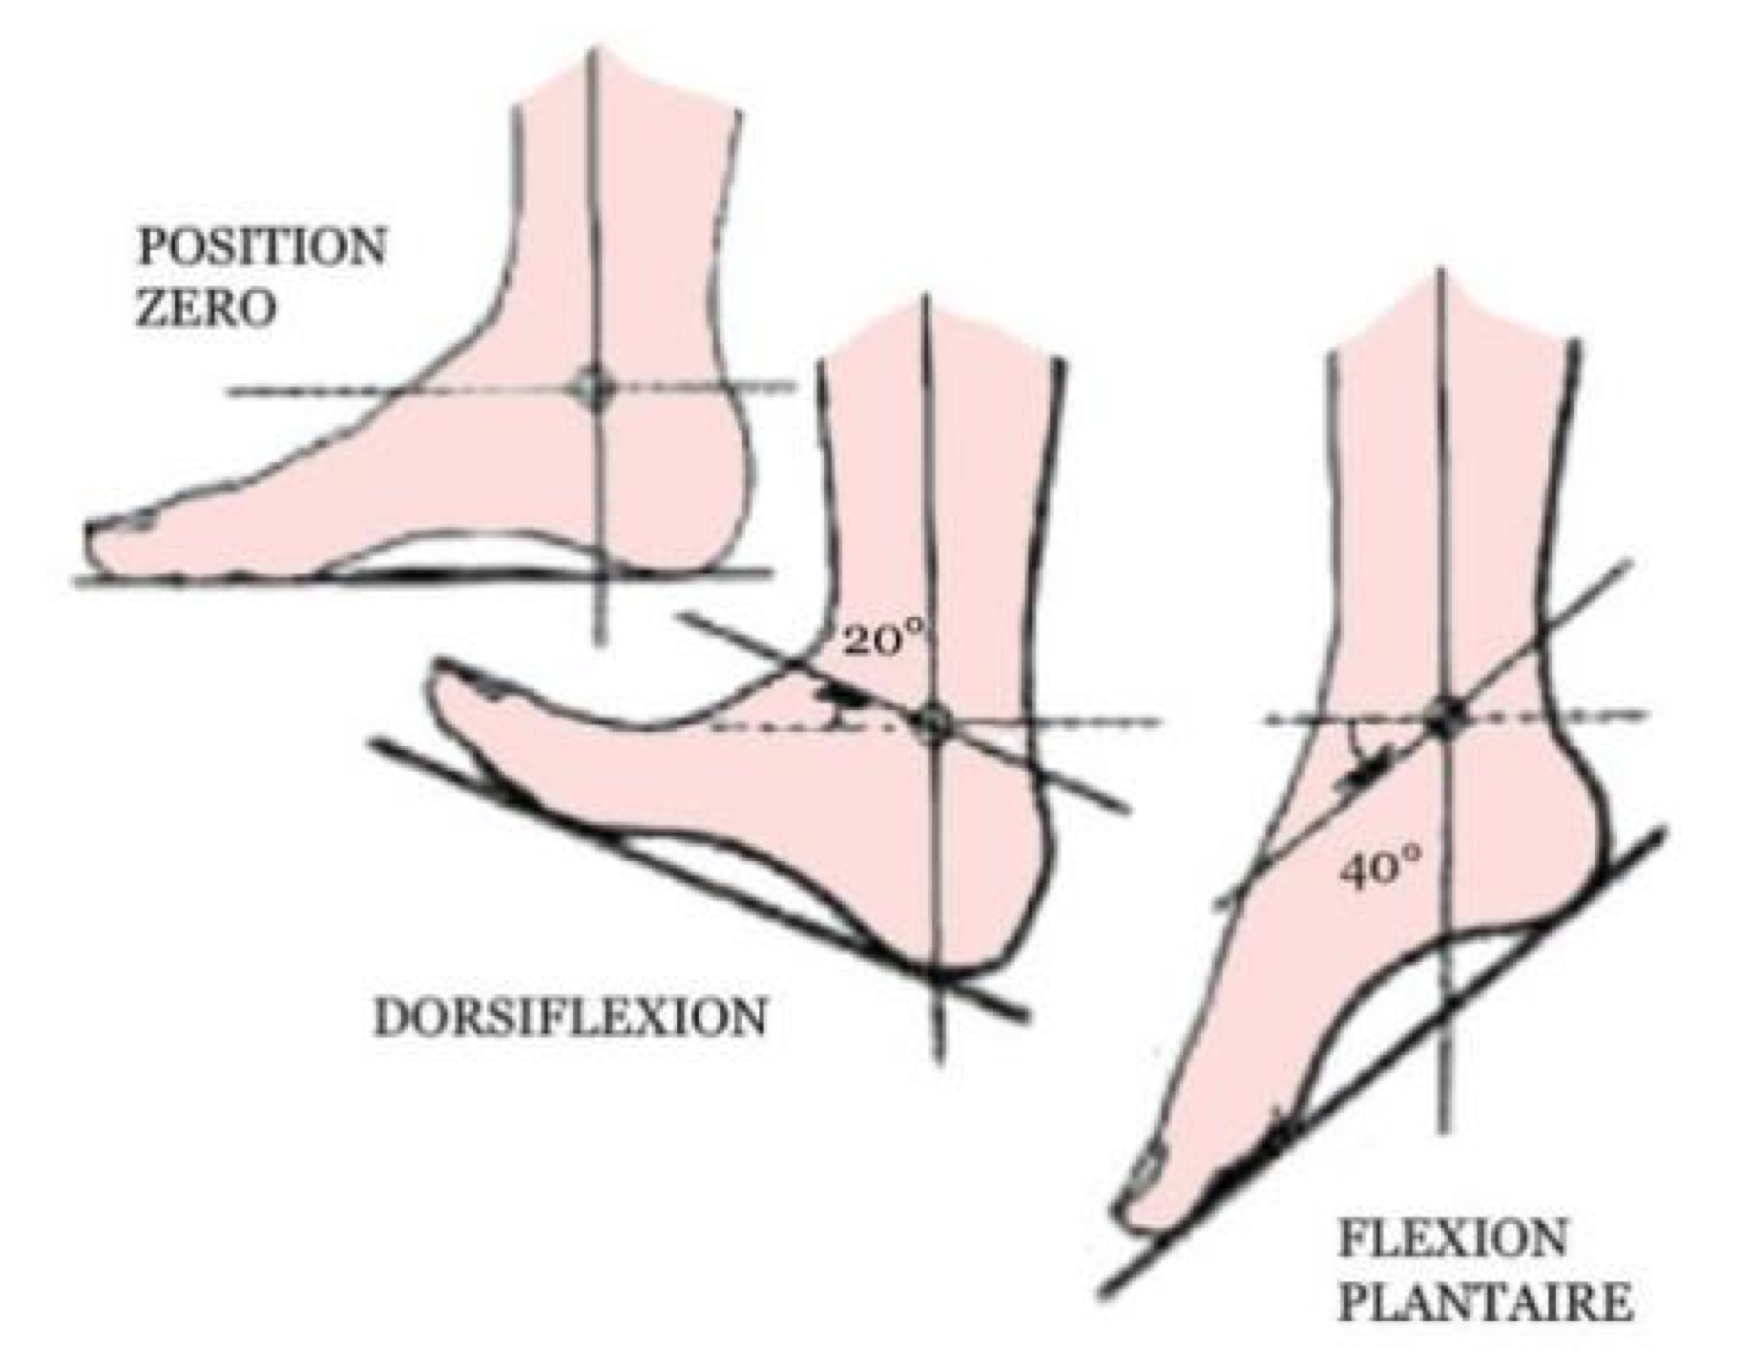
\includegraphics[height=4cm]{human_foot_sagittal.png}}
%     \hfil
%     \subfloat[][]{\label{fig:sagittal_trunk}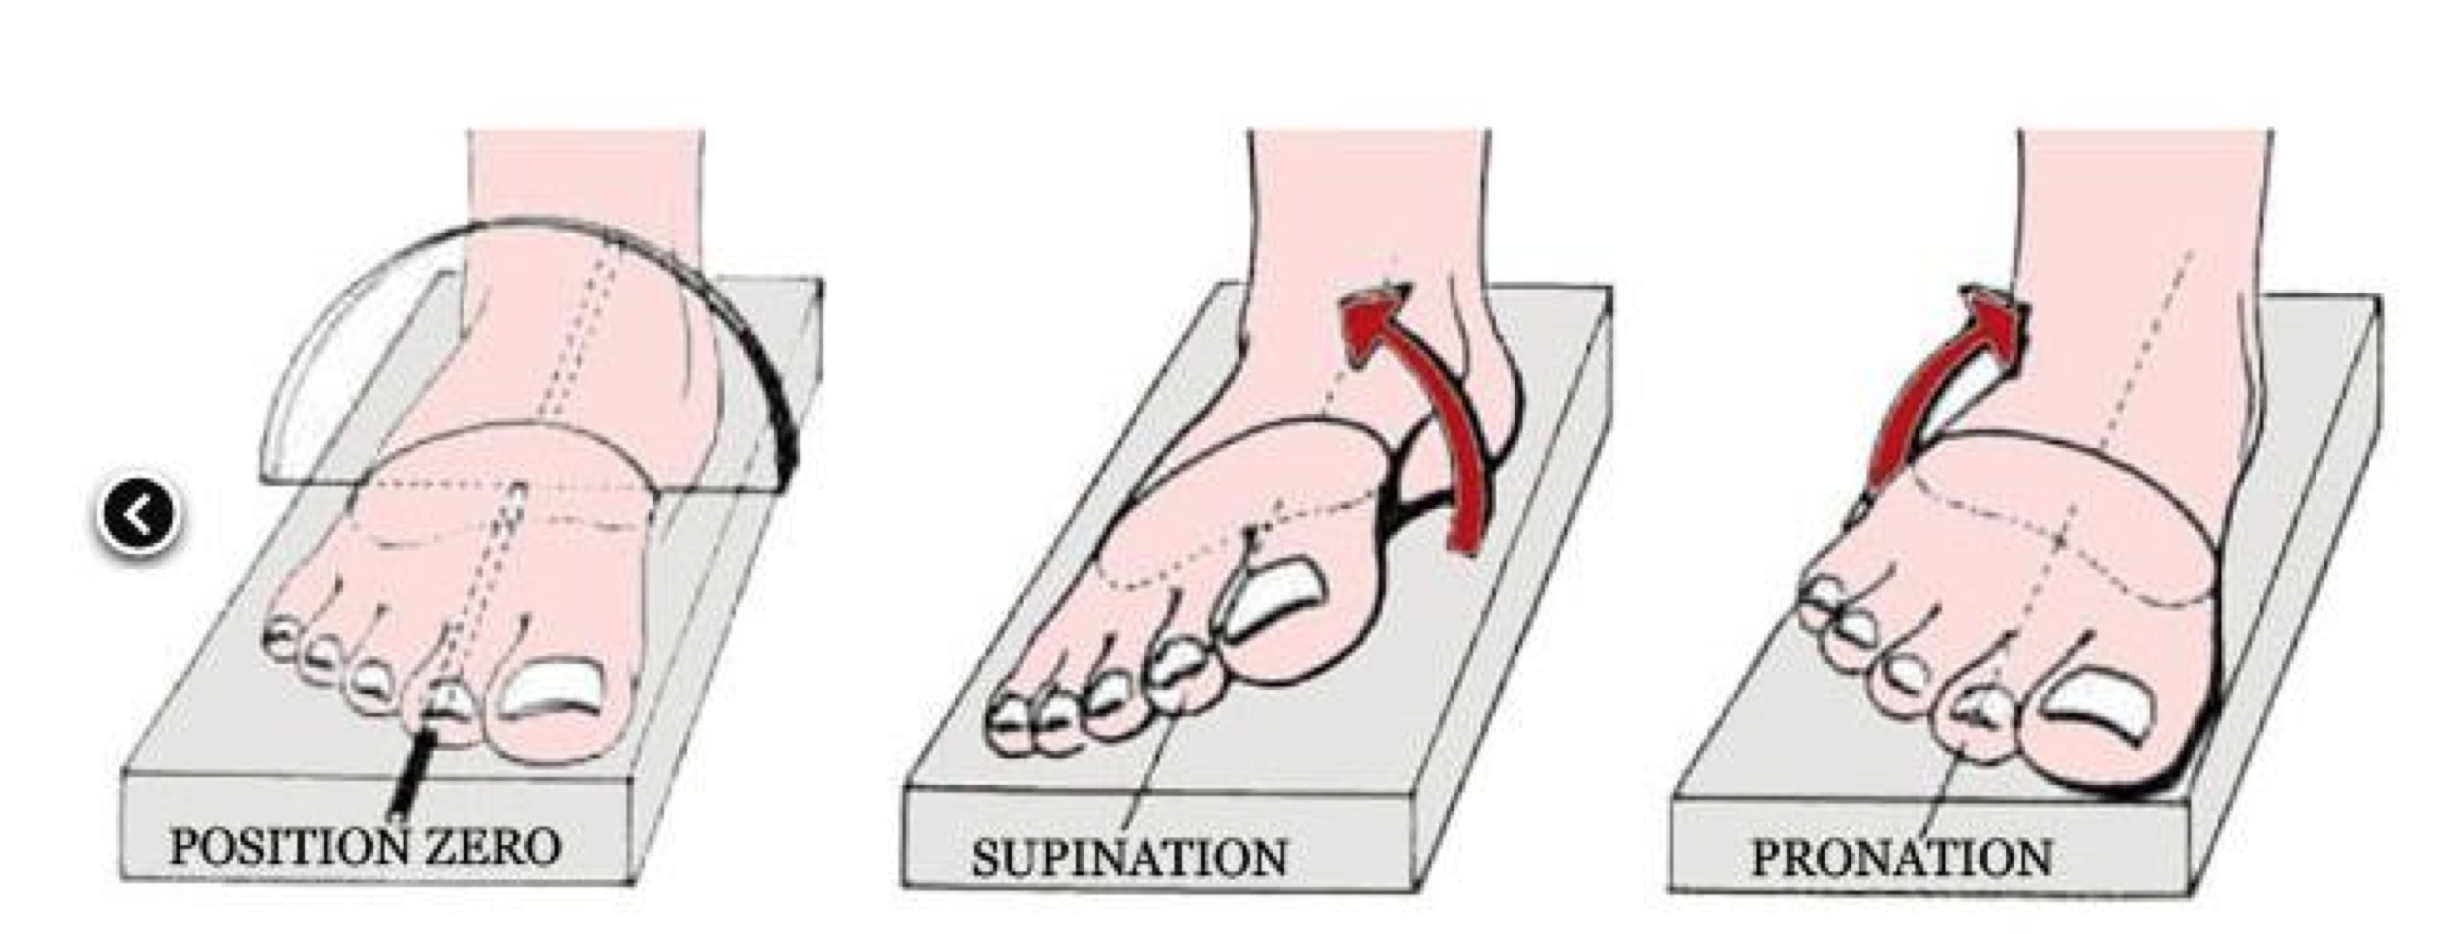
\includegraphics[height=3cm]{human_foot_lateral.png}}
%     \caption{}
%     \label{fig:poppy_torso}
% \end{figure}




\begin{figure}[p]
    \begin{center}
        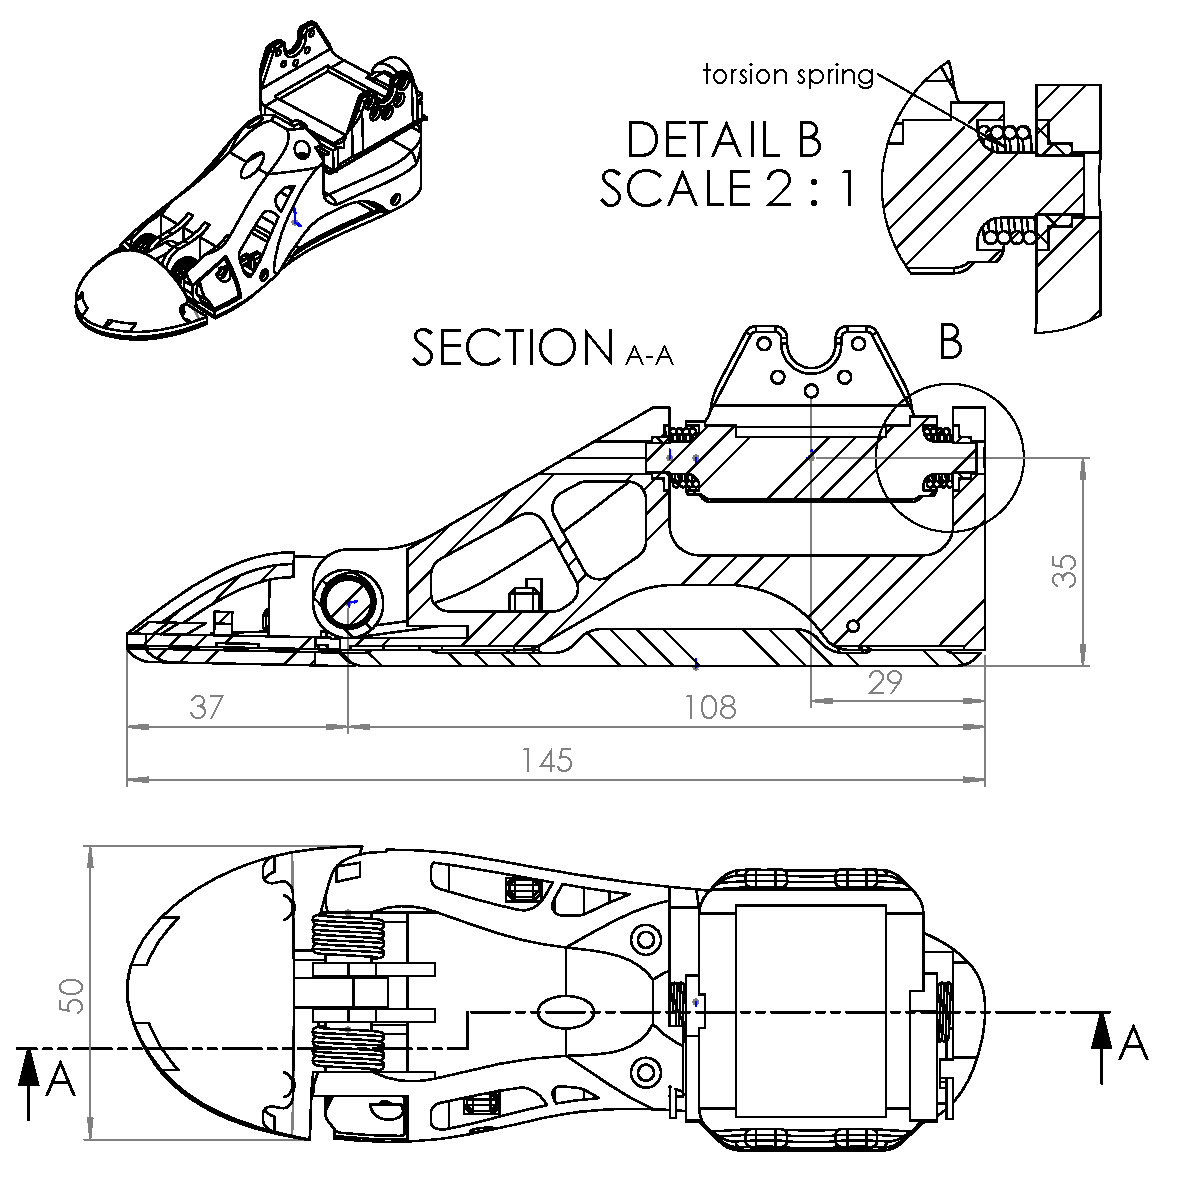
\includegraphics[width=\linewidth]{poppy_foot_v1.pdf}
    \end{center}
    \caption{Caption here}
    \label{fig:poppy-foot-v1-design}
\end{figure}


This design choice as a strong impact on the overall design, because we have lightweight feet, the power requirer to make the leg move is reduced, we can therefore use smaller motors which are also lighter.


\subsection{Legs} % (fold)

Poppy's legs have 6 DoF each, three in the sagittal plane (ankle, knee, hip), one in the horizontal plane (hip) and one in the frontal plane (hip). These joints allow reproducing the main DoF of the human legs. In addition, if we look closely at the human morphology of the femur, it appears that it is inclined of 6 degrees (see \figurename~\ref{fig:human_thigh}). This particularity is reproduced on Poppy's thigh (see \figurename~\ref{fig:poppy_leg_design}).

\begin{figure}[tb]
\centering
    \subfloat[][]{\label{fig:human_thigh}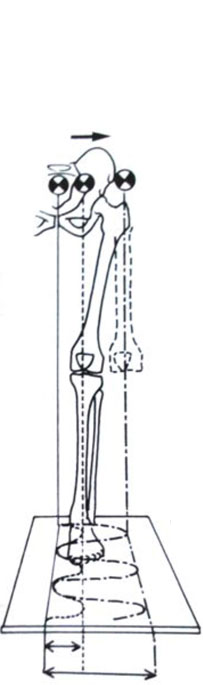
\includegraphics[height=6.5cm]{human_thigh.jpg}}
    \hfil
    \subfloat[][]{\label{fig:model_thigh}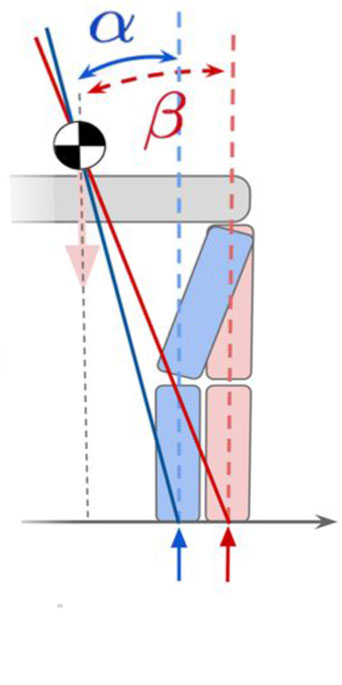
\includegraphics[height=6.5cm]{model_thigh.jpg}}
    \caption{ On \ref{fig:human_thigh}, effect of the bended femur on the human biped locomotion. \ref{fig:model_thigh} Model used for the comparison of the two thighs morphology.}
    \label{fig:poppy_thigh}
\end{figure}


This slight bending makes the feet closer to the projection of the center of gravity and therefore changes the dynamic behavior.
In this thesis we describe both a theoretical model (see appendix REF) and real experiments (see section REF) showing that this bio-inspired thigh allows the reduction of falling speed by almost 60\% (during single support phase) and the decrease of the lateral motion needed for the mass transfer from one foot to the other by 30\% (double support phase).


\begin{figure}[p]
    \begin{center}
        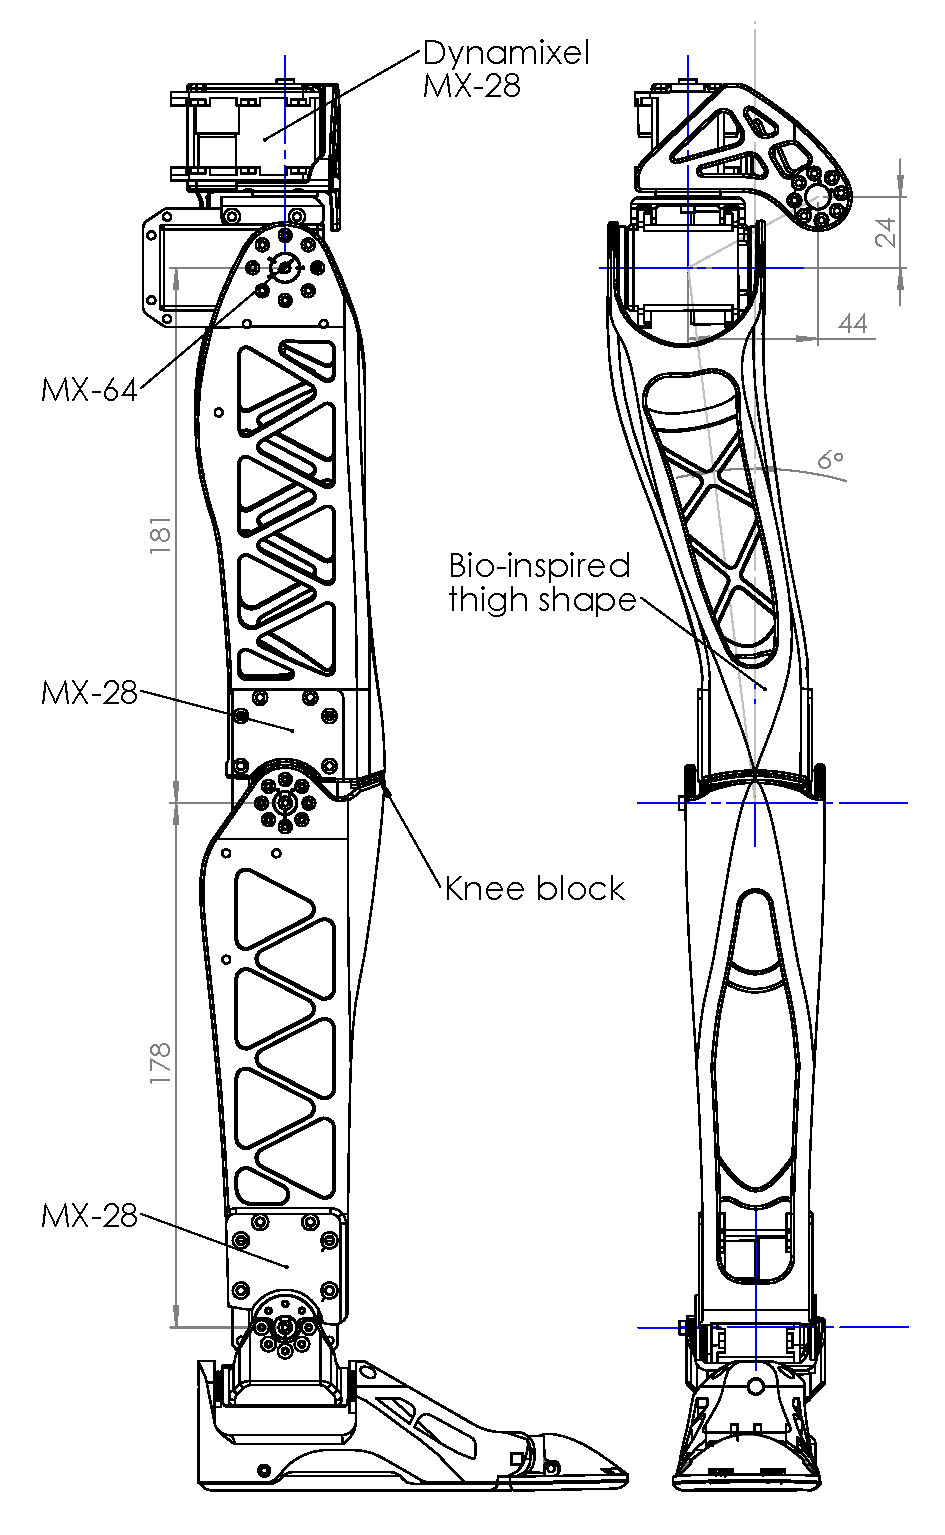
\includegraphics[width=\linewidth]{poppy_leg_design.pdf}
    \end{center}
    \caption{Caption here}
    \label{fig:poppy_leg_design}
\end{figure}


Also, following the principles previously mentioned, the leg design is made to be as light as possible. This was achieved by using truss structure (see section REF) and the minimum required amount of power, involving two Dynamixel MX-28 for the ankle and knee joint, and a Dynamixel MX-64 for the hip joint (see \figurename~\ref{fig:poppy_leg_design}). Yet as explained in section REF, most of our parts have several configurations allowing changing the actuator. Thus it is possible to easily replace the knee actuator by a Dynamixel MX-64 (see \figurename~\ref{REF}).



\section{Hip} % (fold)
\label{sec:hip}


Poppy's small feet increase the challenge of the balance of the robot. Also, to keep the projection of the center of gravity (CoG) inside the support polygon, defined by the feet geometry, it is necessary to control the weight distribution of the robot structure. In particular, we wanted that in its initial upright posture, Poppy stays balanced without any control.

Robotis actuators are among the densest elements in the Poppy platform ($ 1700 kg.m^{3} $) and are the main source of weight ($1.8 kg$). Their spatial distribution represents therefore the major part of the distribution of masses in Poppy. In order to limit the displacement of the mass on the back of the robot, we decided to avoid conventional ball joint assembly for the hip joint such that it is made on most robots based on Robotis motors such as DarwinOP or Acroban (i.e. distributed in a plane parallel to the sagittal plane). Instead, we placed them on the frontal plane as the from left to right stability is greater than the from rear to front stability. By doing so, the hip joint is not a real ball joint anymore. Yet to keep a wide range of motion, we used an original non-symmetrical motor configuration (see \figurename~\ref{fig:poppy_zoom_hip_blueprint}).

This configuration allows:

\begin{itemize}
    \item creating a compact multi-articulated pelvis,
    \item hip rotations (in frontal plane) lead to slight vertical motions of the leg which act as a damper during walking. This damping can be tuned by adjusting the stiffness of the actuator.
    \item it reduces the hip joint lever arm and thus reduces the torque required to maintain position in single support phase,
    \item reduces the distance between rotation axis to stay close from a ball joint,
    \item the resulting V shape frees room to increase the range of motion of the legs in both the frontal and horizontal plane.
\end{itemize}

\begin{figure}[p]
    \begin{center}
        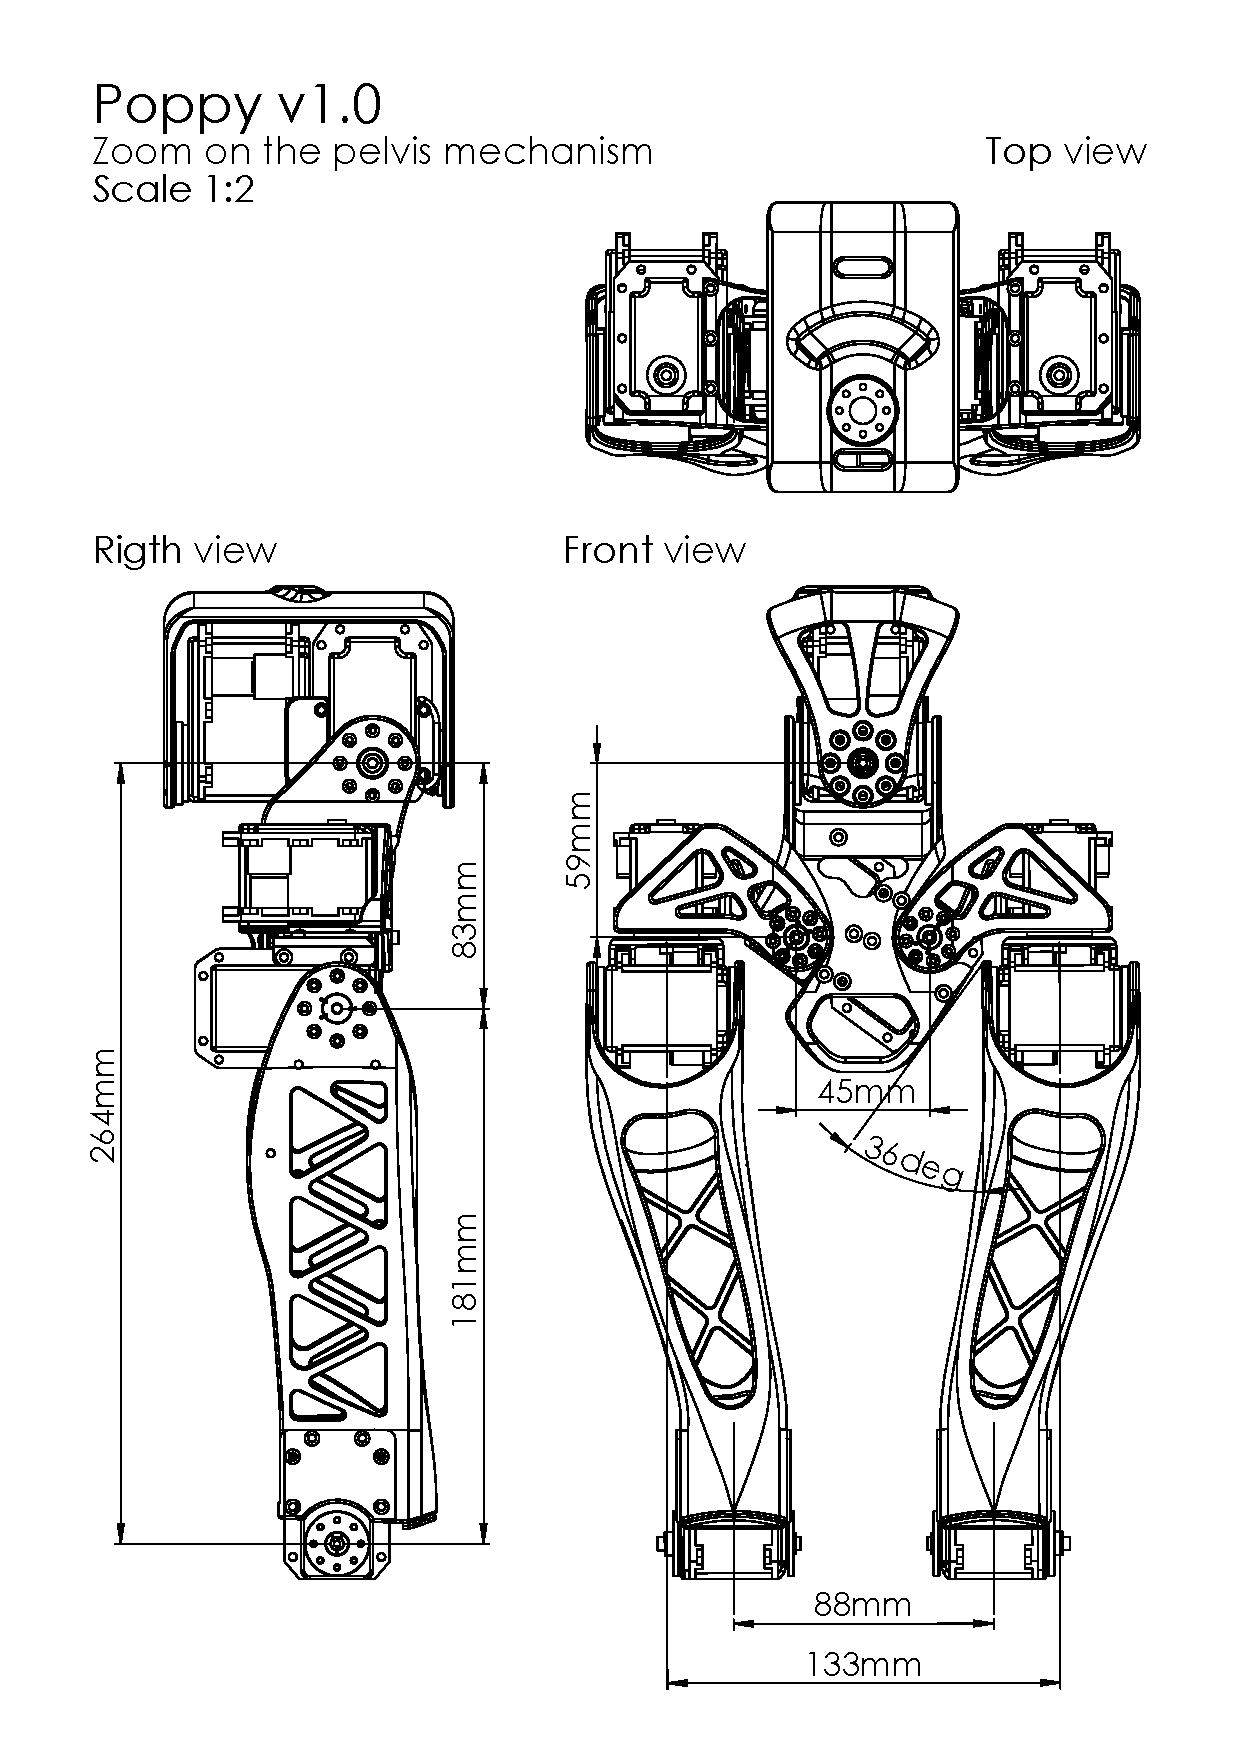
\includegraphics[width=\linewidth]{poppy_zoom_hip_blueprint.pdf}
    \end{center}
    \caption{Caption here}
    \label{fig:poppy_zoom_hip_blueprint}
\end{figure}

In addition, to reduce the shifting of the center of gravity to the back of the robot, the connection with the abs motors is slightly shifted toward the front. By doing so, we .
This permits to keep the CoG in the support polygon and to increase the range of motion of the abs motor when the robot se penche en avant.


\section{Multi-articulated torso} % (fold)

Humanoid robots mostly have a rigid torso without any joint (e.g DarwinOp, Nao, NimbroOP) or few DoFs (e.g. two for Icub, one for HRP-2). However if we look the human trunk and in particular the spine, it has a complex mechanical structure and a large network of dense muscles controlling a very large number of DoFs. It allows for complex motions in several direction while keeping the balance. Its movements are regulated by a complex combination of anticipatory and reactive muscle actions.

Before 1982 and the work of Thorstensson (58), few scientists have really approached the subject. Since, several studies have investigated the activity of the trunk during walking, and showed that the trunk is not only an additional mass but for example participates actively in the walking of Human.
Electromyographics studies showed the importance of the erector spinae muscles in the organization of motor pattern during walking (61),(62),(63) but also of other rhythmic tasks (62). Like the salamander (8), a sequential activation of erector spinae muscles was found (64),(62).
They also show that the trunk is leaning forward and oscillates from 1.5 to 6 deg during walking. In addition, lateral flexion during a gait cycle in the frontal plane promotes the weight shift and opposite rotations of the lumbar and thoracic belts in the horizontal plane allows extend the footstep (59); (60).

\begin{figure}[h]
    \begin{center}
        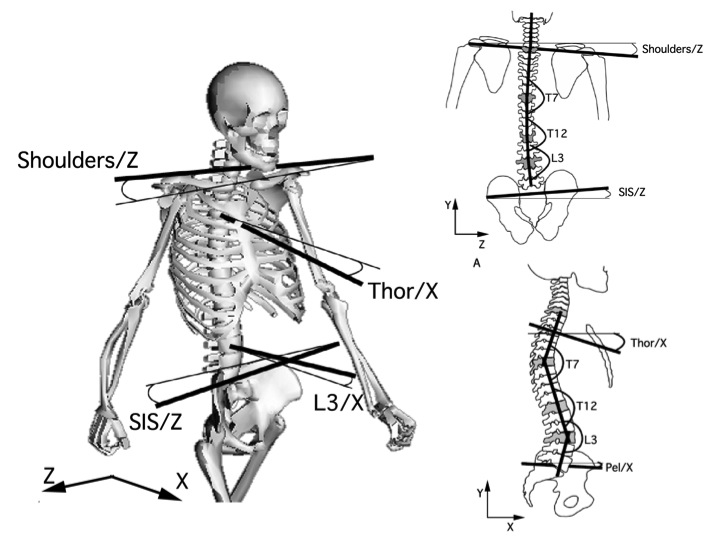
\includegraphics[width=0.7\linewidth]{human_trunk.jpg}
    \end{center}
    \caption{Caption here}
    \label{fig:human_spine_system}
\end{figure}

Thus the trunk of the human is complex and seems to play an important role in the walking of human, essential to all human movements and especially for walking. The movements of the spine can facilitate the transfer of weight from one leg to the other, improve the balance but also participate in the dynamics of the walking.

It seems therefore interesting to enable a humanoid robot trying to explore the role of morphology, to have an articulated trunk in order to evaluate its impact on several task from dynamic walking to physical human-robot interaction. Yet the human trunk is difficult to replicate on a small robot using servo motors and therefore a simplification is needed.

Interestingly, Ceccato~\parencite{ceccatoPlos09} studied the role of trunk during walking and highlighted that there are some places in the spine where the displacements are the most important, i.e. that the apparent high dimensionality of the trunk could be factorized down to a few essential components/dimensions.

Accordingly, it appears we can replicate the essential degrees of freedom of human trunk with two DoFs in the sagittal plane, two in the coronal plane, placed in the pelvis and shoulder/thoracic and one in the horizontal plane placed in the middle of his trunk.

These main degrees of freedom have been first introduced on Acroban~\parencite{Ly2011bio} and continued on Poppy (see \figurename~\ref{fig:poppy_torso}).
Thus Poppy's trunk involves five degree of freedom, we use two Dynamixel MX-64 for the abs as they have to support and move the whole upper body mass, the 3 others joints being less soumis to high constraints are powered by MX-28 (see \figurename~\ref{fig:torso_blueprint}). This multi-articulated trunk allows a wide range of motion that can be useful to explore the role of the torso motion on complex dynamics behavior (balance, walking), grasping and reaching task, or for human-robot interaction, extending the expressive and emotional abilities.

\begin{figure}[p]
\centering
    \subfloat[][]{\label{fig:torso_blueprint}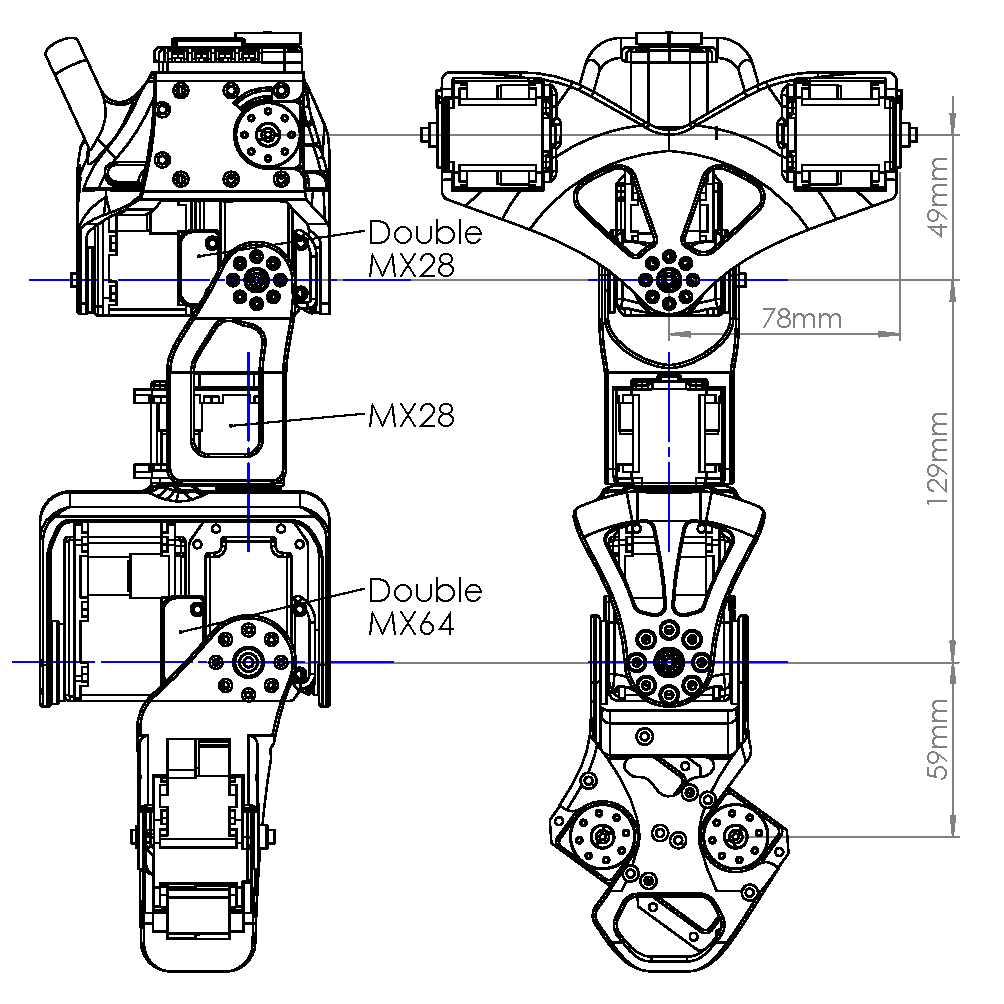
\includegraphics[width=\linewidth]{poppy_torso.pdf}}


    \subfloat[][]{\label{fig:frontal_trunk}\includegraphics[width=0.5\linewidth]{trunk_face.png}}
    \hfil
    \subfloat[][]{\label{fig:sagittal_trunk}\includegraphics[width=0.5\linewidth]{trunk_sagittal.png}}
    \caption{These figures illustrate some morphological features of the Poppy humanoid Robot:\newline a) The Poppy's limbs follow the human being proportion as described in~\parencite{dufour2005biomecanique}.\newline b) and c) Poppy has an articulated trunk of 5 DoFs which allows more natural and fluid motions while improving the user experience during physical interaction and actively participating to the balance of the robot.}
    \label{fig:poppy_torso}
\end{figure}



\subsection{Upper limbs} % (fold)

Poppy's arms were not designed for explore grasping but rather for balancing, expressive and interaction purposes. Thus they only involve the minimum articulations to produce a wide range of motion and they do not involve articulated hands.

A first version of the robot arms involved low-cost AX-12 motors(\$50), but these motors do not allow the same degree of compliance as MX-28 sot the interaction was not smooth enough. We quickly replaced them by MX-28 motors, even if they are more expensive (\$250), powerful and heavy (72gr rather than 50gr), the compliance ability is needed to allow playful physical interaction and demonstration.

This ability was especially useful for the experiments we made with Poppy walking while being socially guided by its hands see videos\footnote{} and experiments on section REF.

Thanks to its multi-articulated structure and its expressive head,

Also these arms combined with the complex spine make Poppy a particularly adapted tool for creating and studying emotions and gesture social communication (see \figurename~\ref{fig:TER_cognitic}). An example of such use has been done by two cognitivist students. Their goals was to study emotion transfer between robot and human. Using Poppy's upper body and pypot recording feature (see section REF), they were able to program a wide range of emotions (see \figurename~\ref{fig:TER_cognitic}).


\begin{figure}[tb]
\centering
    \subfloat[][\url{http://youtu.be/StFIMuyz11M}]{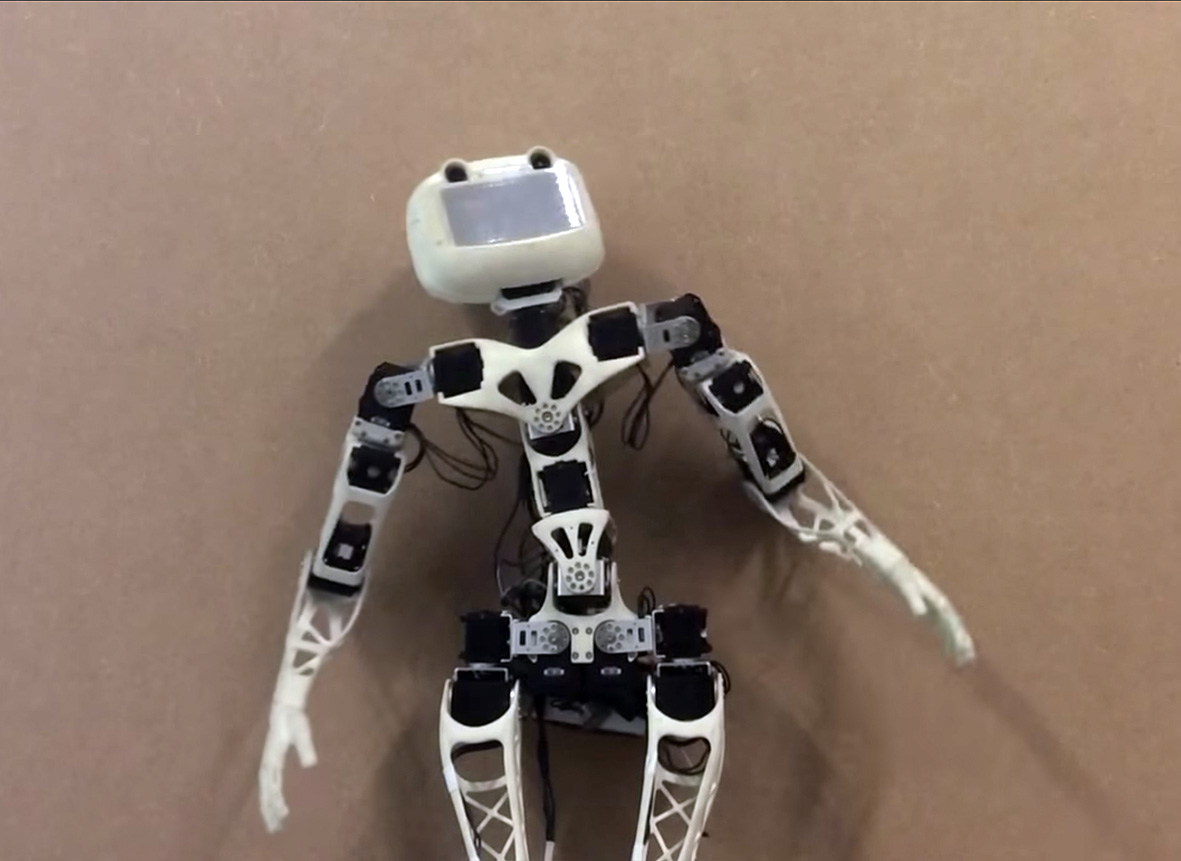
\includegraphics[width=0.45\linewidth]{TER_surprise.jpg}}
    \hfil
    \subfloat[][\url{http://youtu.be/RwCtNwLk10E}]{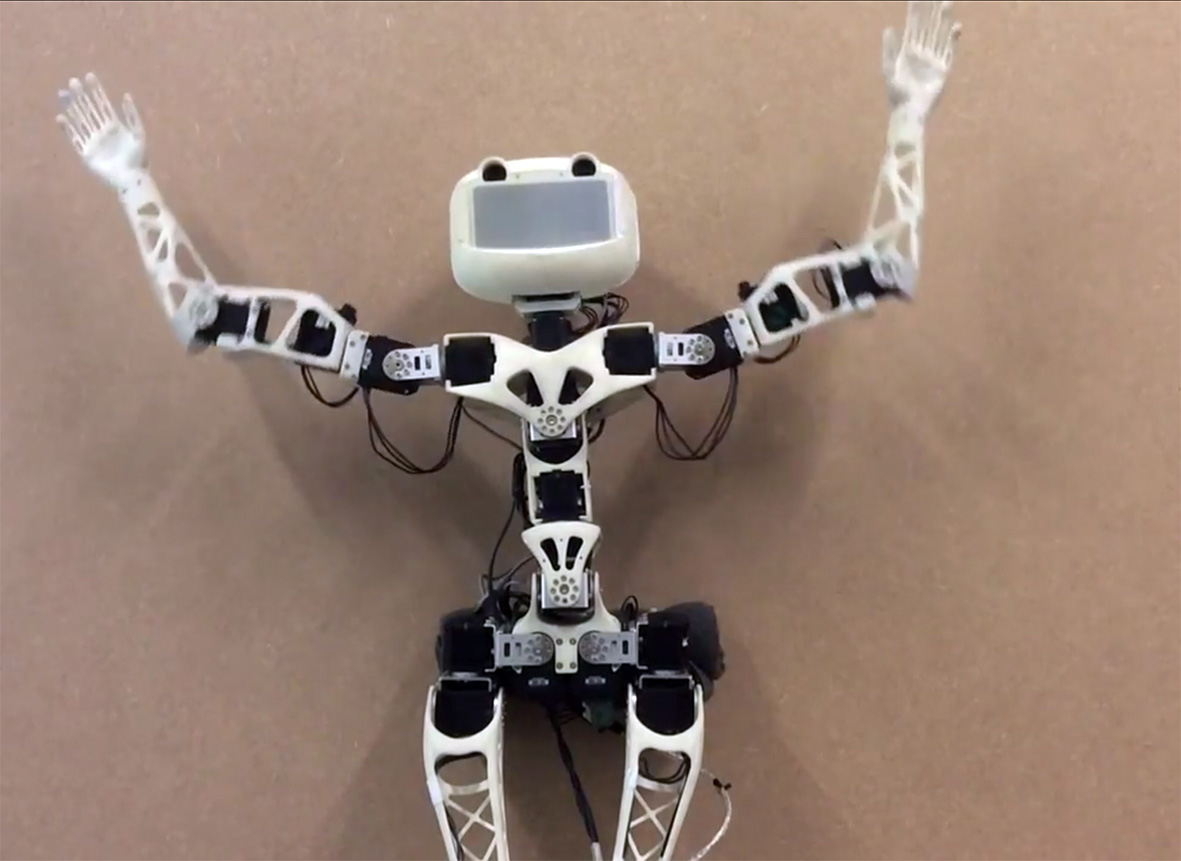
\includegraphics[width=0.45\linewidth]{TER_joy.jpg}}\\
    \subfloat[][\url{http://youtu.be/qrcmLXbpUVo}]{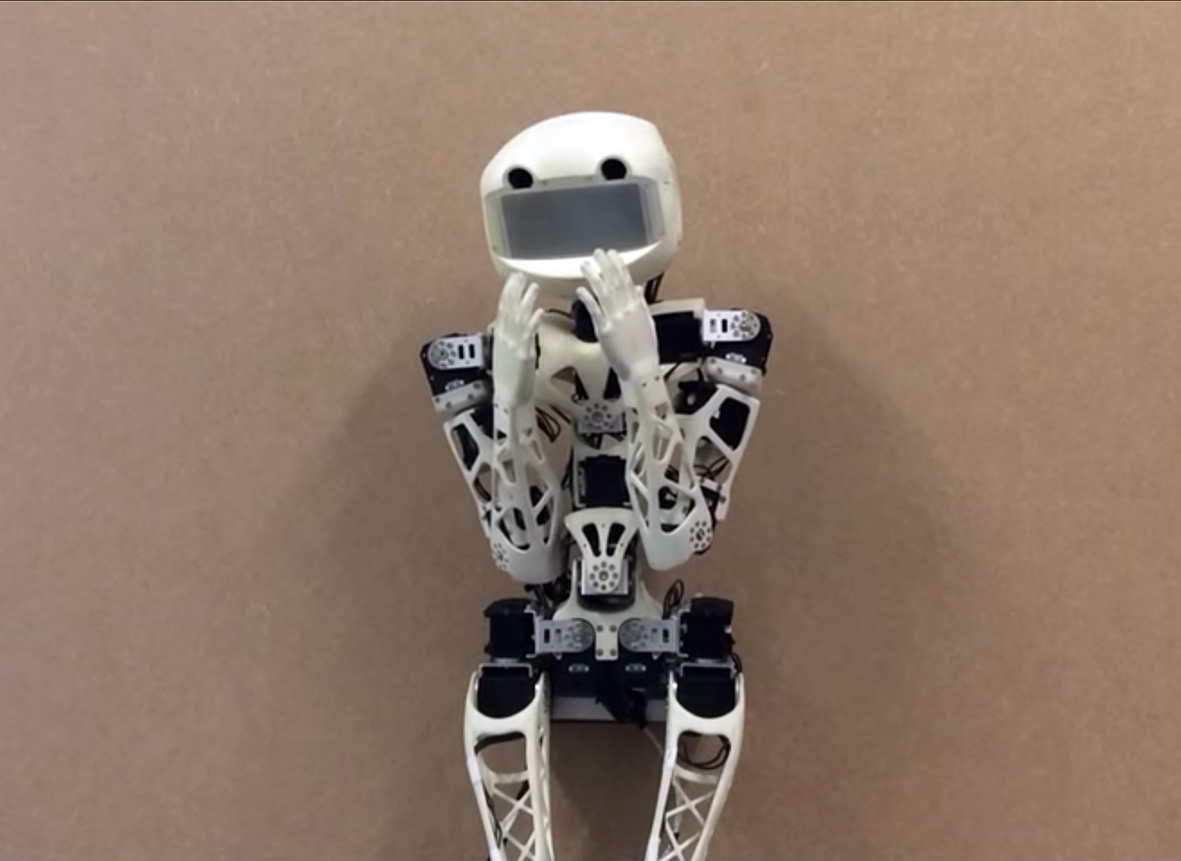
\includegraphics[width=0.45\linewidth]{TER_sad.jpg}}
    \hfil
    \subfloat[][\url{http://youtu.be/ms2niFLevv8}]{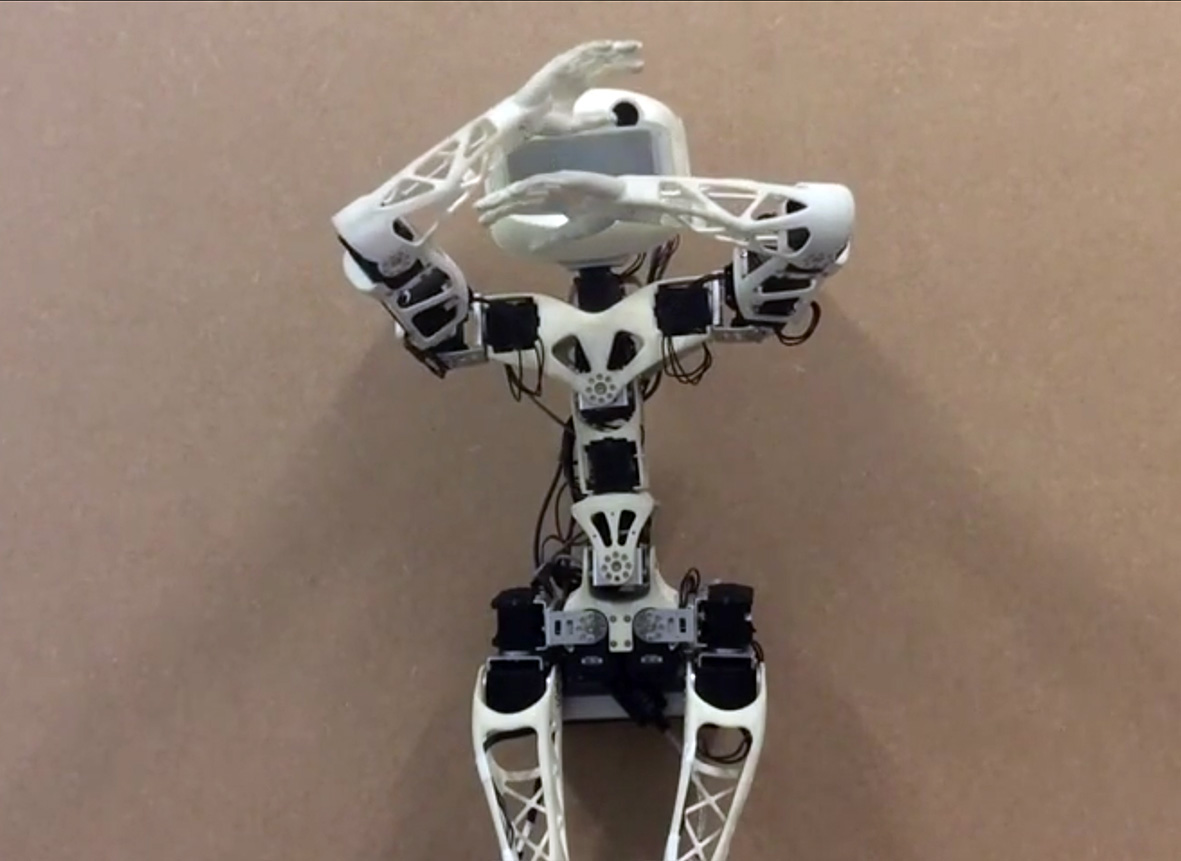
\includegraphics[width=0.45\linewidth]{TER_fear.jpg}}
    \caption{}
    \label{fig:TER_cognitic}
\end{figure}


% \begin{figure}[tb]
%     \begin{center}
%         \includegraphics[width=\linewidth]{arm_block.png}
%     \end{center}
%     \caption{Caption here}
%     \label{fig:figure1}
% \end{figure}




